% Important: If latex complains about unicode characters,
% please use "\usepackage[utf8x]{inputenc}" in your preamble
% You can change the size of the picture by putting it into the construct:
% 1) \resizebox{10cm}{!}{"below picture"} to scale horizontally to 10 cm
% 2) \resizebox{!}{15cm}{"below picture"} to scale vertically to 15 cm
% 3) \resizebox{10cm}{15cm}{"below picture"} a combination of above two
% It is not recomended to use the scale option of the tikzpicture environment.
\resizebox{7cm}{!}{
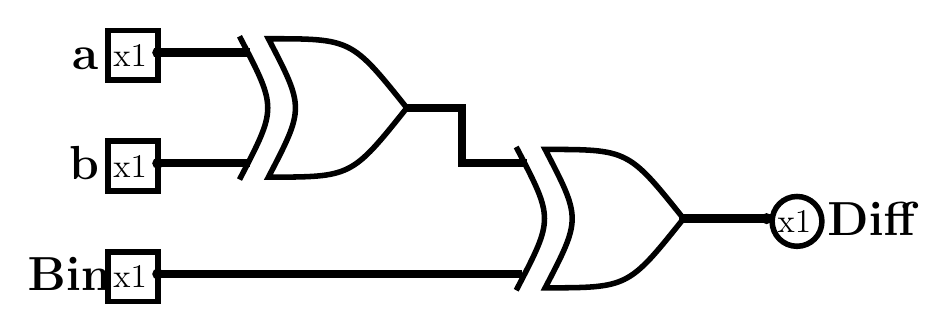
\begin{tikzpicture}[x=1pt,y=-1pt,line cap=rect]
\def\logisimfontA#1{\fontfamily{cmr}{#1}} % Replaced by logisim, original font was "SansSerif"
\definecolor{custcol_0_0_0}{RGB}{0, 0, 0}
\definecolor{custcol_ff_ff_ff}{RGB}{255, 255, 255}
\draw [line width=3.0pt, custcol_0_0_0 ]  (242.0,75.0) -- (272.0,75.0) ;
\draw [line width=3.0pt, custcol_0_0_0 ]  (52.0,15.0) -- (82.0,15.0) -- (84.0,15.0) ;
\draw [line width=3.0pt, custcol_0_0_0 ]  (52.0,55.0) -- (82.0,55.0) -- (84.0,55.0) ;
\draw [line width=2.0pt, custcol_0_0_0 ]  (142.0,35.0) .. controls  (122.0,10.0)  ..  (92.0,10.0) .. controls  (105.0,35.0)  ..  (92.0,60.0) .. controls  (122.0,60.0)  ..  (142.0,35.0) -- cycle ;
\draw [line width=2.0pt, custcol_0_0_0 ]  (82.0,10.0) .. controls  (95.0,35.0)  ..  (82.0,60.0) ;
\draw [line width=2.0pt, custcol_0_0_0]  (283.0,76.0) ellipse (9.0 and 9.0 );
\logisimfontA{\fontsize{12pt}{12pt}\selectfont\node[inner sep=0, outer sep=0, custcol_0_0_0, anchor=base west] at  (276.0,80.0)  {x1};}
\logisimfontA{\fontsize{16pt}{16pt}\fontseries{bx}\selectfont\node[inner sep=0, outer sep=0, custcol_0_0_0, anchor=base west] at  (294.0,81.0)  {Diff};}
\fill [line width=2.0pt, custcol_0_0_0]  (272.0,75.0) ellipse (2.0 and 2.0 );
\draw [line width=3.0pt, custcol_0_0_0 ]  (142.0,35.0) -- (162.0,35.0) -- (162.0,55.0) -- (182.0,55.0) -- (184.0,55.0) ;
\draw [line width=3.0pt, custcol_0_0_0 ]  (52.0,95.0) -- (182.0,95.0) -- (182.0,95.0) ;
\draw [line width=2.0pt, custcol_0_0_0 ]  (242.0,75.0) .. controls  (222.0,50.0)  ..  (192.0,50.0) .. controls  (205.0,75.0)  ..  (192.0,100.0) .. controls  (222.0,100.0)  ..  (242.0,75.0) -- cycle ;
\draw [line width=2.0pt, custcol_0_0_0 ]  (182.0,50.0) .. controls  (195.0,75.0)  ..  (182.0,100.0) ;
\draw [line width=2.0pt, custcol_0_0_0 ]  (34.0,7.0) -- (51.0,7.0) ;
\draw [line width=2.0pt, custcol_0_0_0 ]  (52.0,7.0) -- (52.0,24.0) ;
\draw [line width=2.0pt, custcol_0_0_0 ]  (52.0,25.0) -- (35.0,25.0) ;
\draw [line width=2.0pt, custcol_0_0_0 ]  (34.0,25.0) -- (34.0,8.0) ;
\logisimfontA{\fontsize{12pt}{12pt}\selectfont\node[inner sep=0, outer sep=0, custcol_0_0_0, anchor=base west] at  (36.0,20.0)  {x1};}
\logisimfontA{\fontsize{16pt}{16pt}\fontseries{bx}\selectfont\node[inner sep=0, outer sep=0, custcol_0_0_0, anchor=base west] at  (21.0,21.0)  {a};}
\fill [line width=2.0pt, custcol_0_0_0]  (52.0,15.0) ellipse (2.0 and 2.0 );
\draw [line width=2.0pt, custcol_0_0_0 ]  (34.0,87.0) -- (51.0,87.0) ;
\draw [line width=2.0pt, custcol_0_0_0 ]  (52.0,87.0) -- (52.0,104.0) ;
\draw [line width=2.0pt, custcol_0_0_0 ]  (52.0,105.0) -- (35.0,105.0) ;
\draw [line width=2.0pt, custcol_0_0_0 ]  (34.0,105.0) -- (34.0,88.0) ;
\logisimfontA{\fontsize{12pt}{12pt}\selectfont\node[inner sep=0, outer sep=0, custcol_0_0_0, anchor=base west] at  (36.0,100.0)  {x1};}
\logisimfontA{\fontsize{16pt}{16pt}\fontseries{bx}\selectfont\node[inner sep=0, outer sep=0, custcol_0_0_0, anchor=base west] at  (5.0,101.0)  {Bin};}
\fill [line width=2.0pt, custcol_0_0_0]  (52.0,95.0) ellipse (2.0 and 2.0 );
\draw [line width=2.0pt, custcol_0_0_0 ]  (34.0,47.0) -- (51.0,47.0) ;
\draw [line width=2.0pt, custcol_0_0_0 ]  (52.0,47.0) -- (52.0,64.0) ;
\draw [line width=2.0pt, custcol_0_0_0 ]  (52.0,65.0) -- (35.0,65.0) ;
\draw [line width=2.0pt, custcol_0_0_0 ]  (34.0,65.0) -- (34.0,48.0) ;
\logisimfontA{\fontsize{12pt}{12pt}\selectfont\node[inner sep=0, outer sep=0, custcol_0_0_0, anchor=base west] at  (36.0,60.0)  {x1};}
\logisimfontA{\fontsize{16pt}{16pt}\fontseries{bx}\selectfont\node[inner sep=0, outer sep=0, custcol_0_0_0, anchor=base west] at  (20.0,61.0)  {b};}
\fill [line width=2.0pt, custcol_0_0_0]  (52.0,55.0) ellipse (2.0 and 2.0 );
\end{tikzpicture}
}
